\documentclass{beamer}
\usetheme{Boadilla}
\usepackage{pgfplots}
\usepackage{tikz}
\usetikzlibrary{shapes,arrows,chains}
\usetikzlibrary[calc]
\usepackage{amssymb,amsmath,mathrsfs,stmaryrd,bm,amsthm,amsfonts}
\usepackage{mathtools}
\usepackage{pgfplotstable}
\usepackage{biblatex}
\usepackage{soul}
\addbibresource{../paper/biblio.bib}
\renewcommand{\footnotesize}{\scriptsize}
\usepackage{pifont}
\usetikzlibrary{math}

\DeclareMathOperator{\logit}{logit}
\DeclareMathOperator{\sigmoid}{sigmoid}
\DeclareMathOperator{\abs}{abs}
\DeclareMathOperator{\diag}{diag}
\DeclareMathOperator{\llr}{llr}
\DeclareMathOperator{\lr}{lr}
\DeclareMathOperator{\ilr}{ilr}
\DeclareMathOperator{\ilrl}{ilrl}
\DeclareMathOperator{\e}{e}

\newcommand{\tikzxmark}{
\tikz[scale=0.25] {
    \draw[line width=0.7,color=red,line cap=round] (0,0) to [bend left=6] (1,1);
    \draw[line width=0.7,color=red,line cap=round] (0.2,0.95) to [bend right=3] (0.8,0.05);
}}
\newcommand{\tikzcmark}{
\tikz[scale=0.25] {
    \draw[line width=0.7,color=green,line cap=round] (0.25,0) to [bend left=10] (1,1);
    \draw[line width=0.8,color=green,line cap=round] (0,0.35) to [bend right=1] (0.23,0);
}}

%Information to be included in the title page:
\title[Shapley compositions]{Explaining probabilistic predictions on the simplex\\with Shapley compositions}
\author[Paul-Gauthier Noé]{\textbf{Paul-Gauthier Noé} \inst{1}, Miquel Perelló-Nieto \inst{2},\\Peter Flach \inst{2}, Jean-François Bonastre \inst{1}}
\institute[]{\inst{1} Avignon Université \and \inst{2} University of Bristol}

\date[LIA seminar]
{LIA seminar, Avignon Université\\January 18, 2024}
\begin{document}

\frame{\titlepage}

\section{Introduction}

\begin{frame}
\frametitle{Introduction}

\textbf{Local explanation in machine learning:}

\begin{figure}
  \centering
  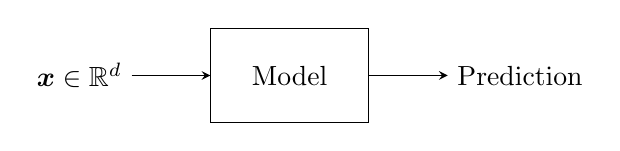
\begin{tikzpicture}
  \node [draw,
	minimum width=2cm,
	minimum height=1.2cm
        ]  (model) {Model};
        \node [left=1cm of model] (x) {$\bm{x}\in\mathbb{R}^d$};
        \node [right=1cm of model] (pred) {Prediction};
        \draw[-stealth] (x.east) -- (model.west);
        \draw[-stealth] (model.east) -- (pred.west);
      \end{tikzpicture}
    \end{figure}
    \textit{Given one instance $\bm{x}$ with $d$ features, what is the contribution/effect of a feature's value on the prediction?}
    

    \begin{center}
      $\neq$ Global explanation
    \end{center}
  \end{frame}

  \begin{frame}
    \frametitle{Introduction}
    Examples of local explanation methods:
    \begin{itemize}
    \item Local Interpretable Model-Agnostic Explanations (LIME) \footfullcite{ribeiro2016should},
    \item Shapley values \footfullcite{vstrumbelj2014explaining} (SHAP toolkit \footfullcite{NIPS2017_7062})
      
    \end{itemize}
  \end{frame}

  \begin{frame}
    \frametitle{Introduction}
    \textbf{Shapley values in cooperative game theory}\footfullcite{shapley1953value}
    \begin{itemize}
    \item Distributes the total payoff among the players.
    \item The unique quantity respecting a set of desired axiomatic properties:
      \begin{itemize}
      \item Linearity:\\
        \begin{equation}
          \phi_{\alpha v + (1-\alpha)w}(i) = \alpha \phi_{v}(i) + (1-\alpha) \phi_{w}(i),
        \end{equation}
        for a player $i$ and two games $v$ and $w$, and for $\alpha \in [0,1]$
      \item Efficiency,
        \begin{equation}
          \sum_{i\in\mathcal{C}} \phi_{v}(i) = v (\mathcal{C}),
        \end{equation}
        (the sum of the value is equal to the total payoff)
      \item Symmetry
      \end{itemize}
    \end{itemize}
  \end{frame}

  \begin{frame}
    \frametitle{Introduction}
    \textbf{Shapley values in machine learning}
    \begin{itemize}
    \pause
    \item Features are treated as players, and the scalar output of the model as the payoff,
    \begin{figure}
  \centering
  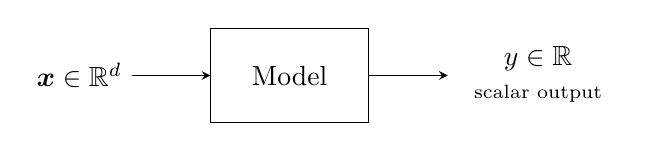
\begin{tikzpicture}
  \node [draw,
	minimum width=2cm,
	minimum height=1.2cm
        ]  (model) {Model};
        \node [left=1cm of model] (x) {$\bm{x}\in\mathbb{R}^d$};
        \node [right=1cm of model] (pred) {\begin{tabular}{c}$y\in\mathbb{R}$\\\scriptsize scalar output\end{tabular}};
        \draw[-stealth] (x.east) -- (model.west);
        \draw[-stealth] (model.east) -- (pred.west);
      \end{tikzpicture}
    \end{figure}
    \pause
    \item Binary classifier, regressor with one-dimensional output \tikzcmark
    \pause
    \item Multiclass classifier \tikzxmark

          ex: The output of a softmax lives on a multidimensional simplex!
        \end{itemize}

  \end{frame}


  \begin{frame}
    \frametitle{Introduction}

\tikzset{%
  every neuron/.style={
    circle,
    draw,
    minimum size=0.5cm
  },
  neuron missing/.style={
    draw=none, 
    scale=2,
    text height=0.333cm,
    execute at begin node=\color{black}$\vdots$
  },
}
    
\begin{figure}
  \centering
  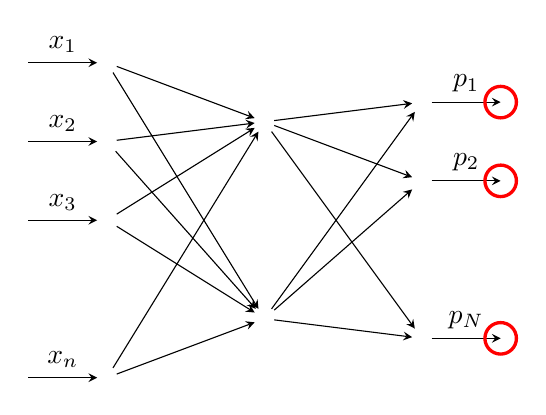
\begin{tikzpicture}[>=stealth]

\foreach \m/\l [count=\y] in {1,2,3,missing,4}
  \node [every neuron/.try, neuron \m/.try] (input-\m) at (0,2.5-\y) {};

\foreach \m [count=\y] in {1,missing,2}
  \node [every neuron/.try, neuron \m/.try ] (hidden-\m) at (2,2-\y*1.25) {};

\foreach \m [count=\y] in {1,2,missing,3}
  \node [every neuron/.try, neuron \m/.try ] (output-\m) at (4,2-\y) {};

\foreach \l [count=\i] in {1,2,3,n}
  \draw [<-] (input-\i) -- ++(-1,0)
    node [above, midway] {$x_\l$};

\foreach \l [count=\i] in {1,n}
  \node [above] at (hidden-\i.north) {};

\foreach \l [count=\i] in {1,2,N}
  \draw [->] (output-\i) -- ++(1,0)
  node [above, midway] {$p_\l$};

\foreach \l [count=\i] in {1,2,N}
  \draw [very thick, color=red] (output-\i)+(1,0) circle (0.2);

\foreach \i in {1,...,4}
  \foreach \j in {1,...,2}
    \draw [->] (input-\i) -- (hidden-\j);

\foreach \i in {1,...,2}
  \foreach \j in {1,...,3}
    \draw [->] (hidden-\i) -- (output-\j);

  \end{tikzpicture}
\end{figure}
\begin{center}
  Some explain the output one-by-one,
\end{center}
\pause

        \begin{center}
          But a probability distribution lives on a simplex,\\
          \textbf{The relative information matter!!}
        \end{center}
        
      \end{frame}

\begin{frame}{Introduction}
  \begin{center}
    The relative information between parts matter!
  \end{center}
  \begin{figure}
    \centering
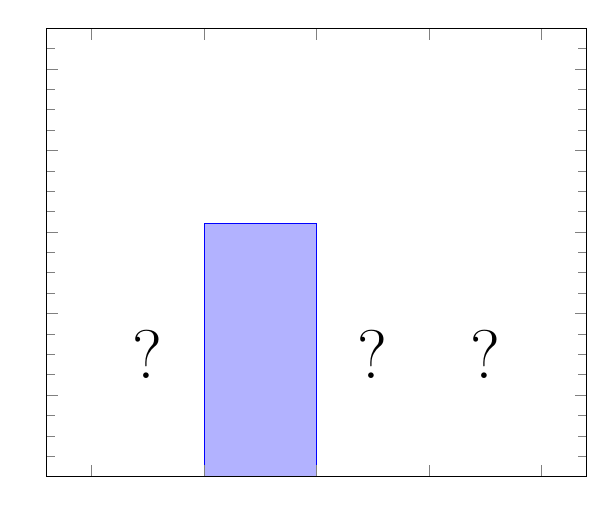
\begin{tikzpicture}
\begin{axis}[
  ymin=0, ymax=55,
  yticklabel=\empty,
  xticklabel=\empty,
    minor y tick num = 3,
    area style,
    ]
    \addplot+[ybar interval,mark=no] plot coordinates { (0, 0) (5, 31) (10, 0) (15, 0) (20, 0) };
    \node[] at (axis cs:2.5,15) {\Huge ?};
    \node[] at (axis cs:12.5,15) {\Huge ?};
    \node[] at (axis cs:17.5,15) {\Huge ?};
\end{axis}
\end{tikzpicture}
  \end{figure}
\end{frame}

\addtocounter{framenumber}{-1}
\begin{frame}{Introduction}
  \begin{center}
    The relative information between parts matter!
  \end{center}
  \begin{figure}
    \centering
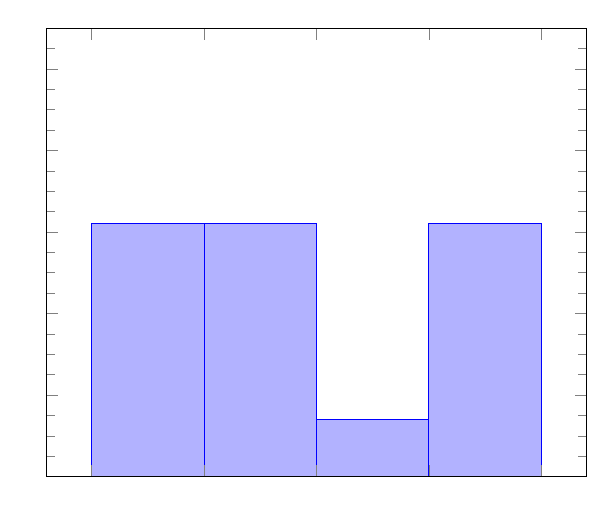
\begin{tikzpicture}
\begin{axis}[
  ymin=0, ymax=55,
  yticklabel=\empty,
  xticklabel=\empty,
    minor y tick num = 3,
    area style,
    ]
\addplot+[ybar interval,mark=no] plot coordinates { (0, 31) (5, 31) (10, 7) (15, 31) (20, 0) };
\end{axis}
\end{tikzpicture}
  \end{figure}
\end{frame}

\addtocounter{framenumber}{-1}
\begin{frame}{Introduction}
  \begin{center}
    The relative information between parts matter!
  \end{center}
  \begin{figure}
    \centering
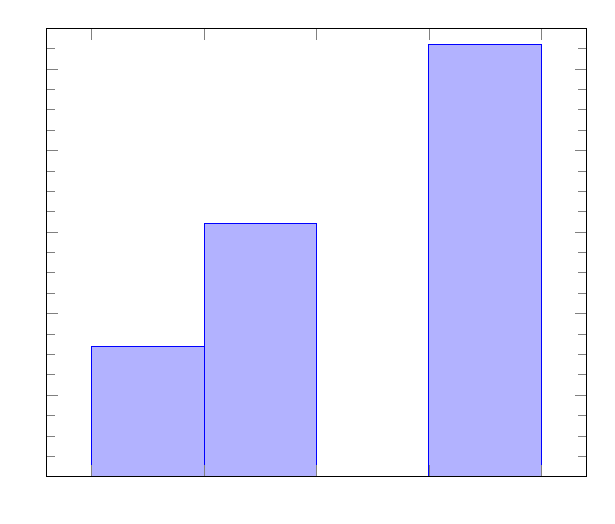
\begin{tikzpicture}
\begin{axis}[
  ymin=0, ymax=55,
  yticklabel=\empty,
  xticklabel=\empty,
    minor y tick num = 3,
    area style,
    ]
\addplot+[ybar interval,mark=no] plot coordinates { (0, 16) (5, 31) (10, 0) (15, 53) (20, 0) };
\end{axis}
\end{tikzpicture}
  \end{figure}
\end{frame}

      
  \begin{frame}
    \frametitle{Introduction}

\tikzset{%
  every neuron/.style={
    circle,
    draw,
    minimum size=0.5cm
  },
  neuron missing/.style={
    draw=none, 
    scale=2,
    text height=0.333cm,
    execute at begin node=\color{black}$\vdots$
  },
}
    
\begin{figure}
  \centering
  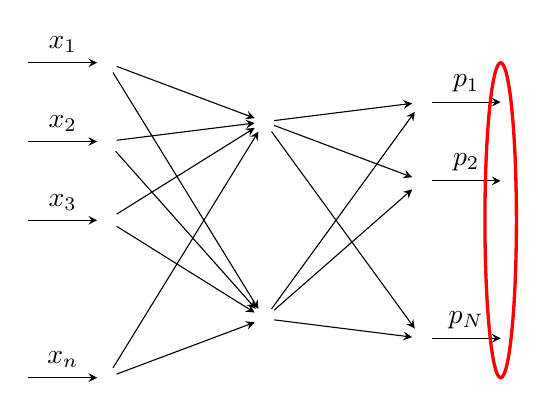
\begin{tikzpicture}[>=stealth]

\foreach \m/\l [count=\y] in {1,2,3,missing,4}
  \node [every neuron/.try, neuron \m/.try] (input-\m) at (0,2.5-\y) {};

\foreach \m [count=\y] in {1,missing,2}
  \node [every neuron/.try, neuron \m/.try ] (hidden-\m) at (2,2-\y*1.25) {};

\foreach \m [count=\y] in {1,2,missing,3}
  \node [every neuron/.try, neuron \m/.try ] (output-\m) at (4,2-\y) {};

\foreach \l [count=\i] in {1,2,3,n}
  \draw [<-] (input-\i) -- ++(-1,0)
    node [above, midway] {$x_\l$};

\foreach \l [count=\i] in {1,n}
  \node [above] at (hidden-\i.north) {};

\foreach \l [count=\i] in {1,2,N}
  \draw [->] (output-\i) -- ++(1,0)
  node [above, midway] {$p_\l$};

\foreach \i in {1,...,4}
  \foreach \j in {1,...,2}
    \draw [->] (input-\i) -- (hidden-\j);

\foreach \i in {1,...,2}
  \foreach \j in {1,...,3}
    \draw [->] (hidden-\i) -- (output-\j);

  \draw [very thick, color=red] (5,-0.5) ellipse (0.2 and 2);
    
  \end{tikzpicture}
\end{figure}
        \begin{center}
          We will explain the probablities all together using the\\
          \emph{Aitchison geometry of the simplex}\footfullcite{aitchison1982,pawlowskymodeling}.
        \end{center}
        
  \end{frame}


  \begin{frame}{Outline}
    \tableofcontents
  \end{frame}
  
\section{The Shapley values in machine learning}


\begin{frame}
\frametitle{The Shapley values in machine learning}

We want to explain a prediction $f(\bm{x})$ on the instance $\bm{x}\in\mathcal{X}\subset\mathbb{R}^d$, where $f:\mathcal{X}\to\mathbb{R}$ is the learned model.
\begin{figure}
  \centering
  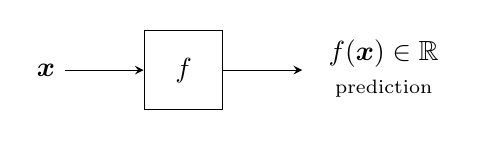
\begin{tikzpicture}
  \node [draw,
	minimum width=1cm,
	minimum height=1cm
        ]  (model) {$f$};
        \node [left=1cm of model] (x) {$\bm{x}$};
        \node [right=1cm of model] (pred) {\begin{tabular}{c}$f(\bm{x})\in\mathbb{R}$\\\scriptsize prediction\end{tabular}};
        \draw[-stealth] (x.east) -- (model.west);
        \draw[-stealth] (model.east) -- (pred.west);
      \end{tikzpicture}
    \end{figure}

\pause
Some notation. Let:
\begin{itemize}
\item $\text{Pr}$ be the probability distribution over $\mathcal{X}$ of the data.
\pause
\item $S\subseteq \mathcal{I}=\{1,2,\dots d\}$ be a subset of indices,
\pause
\item $\bm{x}_S$ refers to an instance $\bm{x}$ restricted to the features indicated by the indices in $S$.
\end{itemize}

\end{frame}

\begin{frame}
  \frametitle{The Shapley values in machine learning}
The \textbf{prediction difference} (knowing only features indexed by $S$):
\begin{equation}
  \begin{aligned}
    \delta_{f,\bm{x},\text{Pr}}: 2^{\mathcal{I}} &\to \mathbb{R},\\
    S &\mapsto \mathbb{E}_\text{Pr}[f(\bm{x})\mid \bm{x}_S] - \mathbb{E}_\text{Pr}[f(\bm{x})],
  \end{aligned}
\end{equation}
where $\mathbb{E}_{\text{Pr}}[f(\bm{x}) \mid \bm{x}_S] = \int_{\bm{x} \in \mathcal{X}}f(\bm{x})\text{Pr}(\bm{x} \mid \bm{x}_S)d\bm{x}$.
\vspace{1cm}

When an instance $\bm{x}$ is observed, the expected value of the prediction is simply $\mathbb{E}[f(\bm{x}) \mid \bm{x}] = f(\bm{x})$. However, when only $\bm{x}_S$ is given with $\mathcal{S} \neq \mathcal{I}$, there is uncertainty about the non-observed features and we therefore compute the expected prediction given $\bm{x}_S$.
\end{frame}

\begin{frame}
\frametitle{The Shapley values in machine learning}
  
The \textbf{contribution} of the feature indexed by $i \notin S$ in the prediction $f(\bm{x})$ given the known features indexed by $S$ is given by:
\begin{equation}
  \label{eq:contrib}
  c_{f,\bm{x},\text{Pr}}(i,\bm{X}_S) = \delta_{f,\bm{x},\text{Pr}}(\bm{X}_{S\cup\{i\}}) - \delta_{f,\bm{x},\text{Pr}}(\bm{X}_S),
\end{equation}

This measures the contribution of the $i$th features with a particular \emph{coalition} of features indexed by $S$.
\end{frame}

\begin{frame}
  \frametitle{The Shapley values in machine learning}
  
 The whole contribution of the $i$th feature is computed by averaging this quantity over all possible coalitions of features as follows:
\begin{equation}
  \phi_{f,\bm{x},\text{Pr}}(i) = \frac{1}{d!} \sum_{\pi}c_{f,\bm{x},\text{Pr}}(i,\pi^{<i}_{\bm{X}}),
\end{equation}
where $\pi$ is a permutation of the set $\mathcal{I}$ of indexes and $\pi^{<i}_{\bm{X}}$ is the features of $\bm{X}$ coming before the $i$th feature in the ordering given by $\pi$.
\pause
\begin{center}
  This quantity is known as the {\Large\textbf{Shapley value}} for the $i$th feature.
\end{center}

\end{frame}

\begin{frame}
  \frametitle{The Shapley values in machine learning}
  
  It comes from cooperative game theory and is known to be the only quantity respecting a set of desired axiomatic properties \footfullcite{shapley1953value}.
  \begin{itemize}
    \pause
\item Linearity with respect to the model ($\alpha, \beta \in \mathbb{R}$): $\phi_{\alpha f +\beta g}(i) = \alpha \phi_f(i) + \beta \phi_g(i)$,
    \pause
\item The ``centered'' learned model is additively separable with respect to the Shapley values:
\begin{equation}
  f(\bm{x})-\mathbb{E}_{\text{Pr}}[f(\bm{X})] = \sum_{i=1}^{d} \phi_f(i),
\end{equation}
which is known as the \emph{efficiency} property.
    \pause
\item Symmetry
\end{itemize}

\end{frame}

\begin{frame}
  \frametitle{The Shapley values in machine learning}
  Example of explanation:
  \begin{figure}
    \centering
    \includegraphics[width=\linewidth]{figures/example_from_shap}
    \caption{Explanation of the probability for the class Setosa for a flower from the Iris dataset. The classifier is an SVM with radial basis function and pairwise coupling. {\tiny Image from \url{https://github.com/shap/shap/tree/master}.}}
  \end{figure}

  Efficiency: $\underbrace{f(\bm{x})}_{\text{prediction}}-\underbrace{\mathbb{E}_{\text{Pr}}[f(\bm{X})]}_{\text{base value}} = \sum_{i=1}^{d} \phi_f(i),$
  \vspace{1cm}
  
  Note that the Shapley explanation is ran in the \emph{logit} domain!
  
\end{frame}


  \begin{frame}
  \frametitle{The Shapley values in machine learning}

\tikzset{%
  every neuron/.style={
    circle,
    draw,
    minimum size=0.5cm
  },
  neuron missing/.style={
    draw=none, 
    scale=2,
    text height=0.333cm,
    execute at begin node=\color{black}$\vdots$
  },
}
    
\begin{figure}
  \centering
  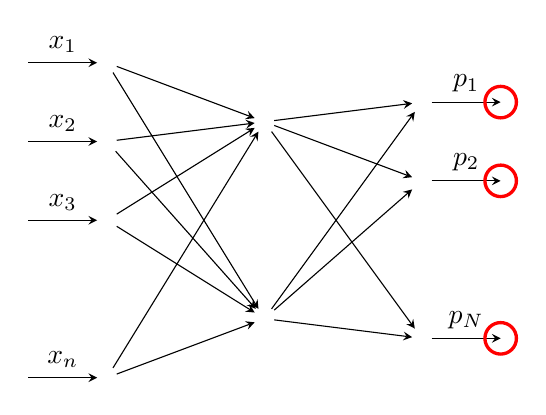
\begin{tikzpicture}[>=stealth]

\foreach \m/\l [count=\y] in {1,2,3,missing,4}
  \node [every neuron/.try, neuron \m/.try] (input-\m) at (0,2.5-\y) {};

\foreach \m [count=\y] in {1,missing,2}
  \node [every neuron/.try, neuron \m/.try ] (hidden-\m) at (2,2-\y*1.25) {};

\foreach \m [count=\y] in {1,2,missing,3}
  \node [every neuron/.try, neuron \m/.try ] (output-\m) at (4,2-\y) {};

\foreach \l [count=\i] in {1,2,3,n}
  \draw [<-] (input-\i) -- ++(-1,0)
    node [above, midway] {$x_\l$};

\foreach \l [count=\i] in {1,n}
  \node [above] at (hidden-\i.north) {};

\foreach \l [count=\i] in {1,2,N}
  \draw [->] (output-\i) -- ++(1,0)
  node [above, midway] {$p_\l$};

\foreach \l [count=\i] in {1,2,N}
  \draw [very thick, color=red] (output-\i)+(1,0) circle (0.2);

\foreach \i in {1,...,4}
  \foreach \j in {1,...,2}
    \draw [->] (input-\i) -- (hidden-\j);

\foreach \i in {1,...,2}
  \foreach \j in {1,...,3}
    \draw [->] (hidden-\i) -- (output-\j);

  \end{tikzpicture}
\end{figure}
\begin{center}
  Some explain the output one-by-one,
\end{center}

        \begin{center}
          But a probability distribution lives on a simplex,\\
          \textbf{The relative information matter!!}
        \end{center}
        
      \end{frame}

      
  \begin{frame}
  \frametitle{The Shapley values in machine learning}

\tikzset{%
  every neuron/.style={
    circle,
    draw,
    minimum size=0.5cm
  },
  neuron missing/.style={
    draw=none, 
    scale=2,
    text height=0.333cm,
    execute at begin node=\color{black}$\vdots$
  },
}
    
\begin{figure}
  \centering
  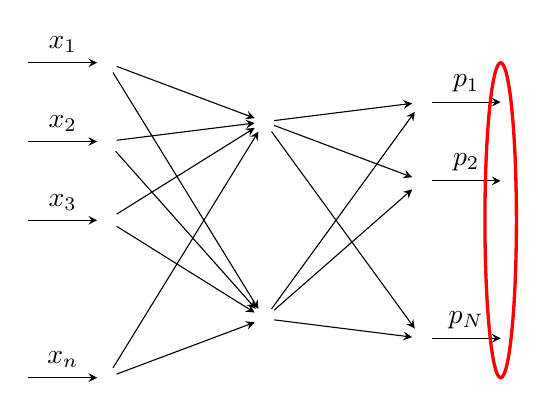
\begin{tikzpicture}[>=stealth]

\foreach \m/\l [count=\y] in {1,2,3,missing,4}
  \node [every neuron/.try, neuron \m/.try] (input-\m) at (0,2.5-\y) {};

\foreach \m [count=\y] in {1,missing,2}
  \node [every neuron/.try, neuron \m/.try ] (hidden-\m) at (2,2-\y*1.25) {};

\foreach \m [count=\y] in {1,2,missing,3}
  \node [every neuron/.try, neuron \m/.try ] (output-\m) at (4,2-\y) {};

\foreach \l [count=\i] in {1,2,3,n}
  \draw [<-] (input-\i) -- ++(-1,0)
    node [above, midway] {$x_\l$};

\foreach \l [count=\i] in {1,n}
  \node [above] at (hidden-\i.north) {};

\foreach \l [count=\i] in {1,2,N}
  \draw [->] (output-\i) -- ++(1,0)
  node [above, midway] {$p_\l$};

\foreach \i in {1,...,4}
  \foreach \j in {1,...,2}
    \draw [->] (input-\i) -- (hidden-\j);

\foreach \i in {1,...,2}
  \foreach \j in {1,...,3}
    \draw [->] (hidden-\i) -- (output-\j);

  \draw [very thick, color=red] (5,-0.5) ellipse (0.2 and 2);
    
  \end{tikzpicture}
\end{figure}
        \begin{center}
          We will explain the probablities all together using the\\
          \emph{Aitchison geometry of the simplex}.
        \end{center}
        
  \end{frame}

\section{Compositional data analysis}

\begin{frame}{Compositional data analysis}
  \begin{minipage}{0.49\textwidth}
    \begin{figure}
      \centering
      \includegraphics[width=0.6\textwidth]{figures/basalt.jpg}
      \caption{A piece of basalt}
    \end{figure}
  \end{minipage}
    \begin{minipage}{0.5\textwidth}
      Composition:
      \begin{itemize}
      \item 35\% of pyroxene,
      \item 50\% of plagioclase,
      \item 12\% of olivine,
      \item 3\% of magnetite.  
      \end{itemize}
      \vspace{0.4cm}
      $\bm{x} = [35,50,12,3]^T$,\\
      \vspace{0.2cm}
      $\displaystyle \sum_{i} x_i = 100\%$.
  \end{minipage}
\end{frame}


\begin{frame}{Compositional data analysis}
  A composition lives on a simplex:
    \vspace{-0.3cm}
    \begin{equation}
      \mathcal{S}^N = \Big\{ \bm{x} = [x_1, x_2,\dots x_{N}]^T \in \mathbb{R}^N \mid \forall i\in\llbracket 1,N \rrbracket, x_i>0 \text{~and~} \sum_{i=1}^{N} x_i = k \Big\},
    \end{equation}
    \vspace{-0.3cm}
    \begin{minipage}{0.53\textwidth}
      \begin{figure}
        \centering
        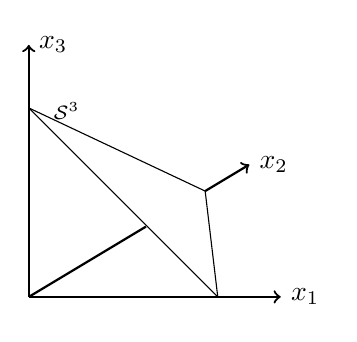
\begin{tikzpicture}[scale=0.8]

\draw [->,thick] (0,0) -- (0,4) node [right] {$x_3$};

\draw [->,thick] (0,0) -- (4,0) node [right] {$x_1$};

\draw [thick] (0,0) -- (1.86,1.116);

\draw [->,thick] (2.8,1.68) -- (3.5,2.1) node [right] {$x_2$};

\draw [] (0,3) -- (3,0);

\draw [] (0,3) -- (2.8,1.68);

\draw [] (3,0) -- (2.8,1.68);

\draw [] (0.6,2.95) node {\scriptsize $\mathcal{S}^3$};

% \draw [blue,dashed,semithick] (0,0) -- (1.5,1.5);
% %\draw [dotted,blue] (1.5,1.5) -- (1.88,1.88);
% \draw [blue,dashed,semithick] (1.88,1.88) -- (4,4);
% \draw [blue] (1.88,1.88) node {\tiny\textbullet};
% \node[minimum size=2pt,blue,fill,draw,circle,inner sep=0pt] () at (1.88,1.88){};
% \draw [blue] (1.91,1.68) node {\scriptsize $\mathcal{C}(\bm{w})$};

% \draw [blue] (3,3) node {\tiny\textbullet};
% \node[minimum size=2pt,blue,fill,draw,circle,inner sep=0pt] () at (3,3){};
% \draw [blue] (3.03,2.8) node {\scriptsize $\bm{w}$};

% \draw [blue,dashed,semithick] (0,0) -- (1.123,1.865);
% %\draw [dotted,blue] (1.123,1.865) -- (1.2,1.99);
% \draw [blue,dashed,semithick] (1.2,1.99) -- (2.83,4.7);
% %\draw [blue] (1.2,1.99) node {\tiny\textbullet};
% \node[minimum size=2pt,blue,fill,draw,circle,inner sep=0pt] () at (1.2,1.99){};


% \draw [blue,dashed,semithick] (2.8,0.49) -- (5.55,0.98);
% %\draw [dotted,blue] (2.55,0.45) -- (2.8,0.49);
% \draw [blue,dashed,semithick] (0,0) -- (2.55,0.45);
% \node[minimum size=2pt,blue,fill,draw,circle,inner sep=0pt] () at (2.8,0.49){};


\end{tikzpicture}

%%% Local Variables:
%%% mode: latex
%%% TeX-master: "../../../main"
%%% TeX-engine: xetex
%%% End:


        \caption{Two dimensional simplex as the sample space of three-parts compositional data.}
      \end{figure}
    \end{minipage}
    \begin{minipage}{0.45\textwidth}
  Exemples of compositional data:
  \begin{itemize}
  \item vectors of percentages,
  \item vectors of concentrations,
  \item \textbf{discrete probability distributions} (probability simplex: $k=1$).
    \end{itemize}
    \end{minipage}    
\end{frame}
  
\begin{frame}{Compositional data analysis}
  \begin{center}
    {\large
      \textbf{The Aitchison geometry of the simplex} gives to the simplex an\\
      \textbf{Euclidean vector space} structure.
    } \footfullcite{aitchison1986statistical,aitchison2001}\\
  \end{center}
  \vspace{0.5cm}
  {\footnotesize
    $\bm{x},\bm{y} \in \mathcal{S}^N$ and $\alpha \in \mathbb{R}$,
  \begin{itemize}
\item perturbation: $\bm{x}\oplus \bm{y} = \mathcal{C}\left([x_1y_1,\dots x_{N}y_{N}]\right)$,
    \item powering: $\alpha \odot \bm{x} = \mathcal{C}\left([x_{1}^{\alpha},\dots x_{N}^{\alpha}]\right)$,
    \item inner product: $\displaystyle \langle \bm{x},\bm{y} \rangle_a = \frac{1}{2N}\sum_{i=1}^{N} \sum_{j=1}^{N} \log \frac{x_i}{x_j}\log \frac{y_i}{y_j}$
  \end{itemize}
  where, $\mathcal{C}\left(\bm{x} \right) = \left[ \frac{x_1}{\lVert \bm{x} \rVert_1}, \frac{x_2}{\lVert \bm{x} \rVert_1} ,\dots \frac{x_N}{\lVert \bm{x} \rVert_1} \right]^T$ is the \emph{closure} operator.
  }
\end{frame}


\begin{frame}{Compositional data analysis}

  \textbf{Cartesian coordinate system and the ILR transformation}
\begin{equation}
    \tilde{\bm{p}}=\ilr(\bm{p}) = \left[\underbrace{\langle \bm{p}, \bm{e}^{(1)} \rangle_a}_{\color{blue} \tilde{\bm{p}}_1} , \underbrace{\langle \bm{p}, \bm{e}^{(2)} \rangle_a}_{\color{magenta} \tilde{\bm{p}}_2},\dots \underbrace{\langle \bm{p}, \bm{e}^{(N-1)} \rangle_a}_{\color{teal} \tilde{\bm{p}}_{N-1}}  \right]^T \in \mathbb{R}^{N-1}.
  \end{equation}
  where $\{\bm{e}^{(i)}\}_{1\leq i \leq N}$ forms an \emph{Aitchison} orthonormal basis on the simplex\footfullcite{egozcue2003isometric}.
  \begin{figure}
    \begin{minipage}{0.39\textwidth}
      \centering
      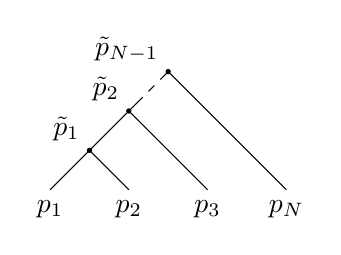
\begin{tikzpicture}[scale=1]
  \draw (0,0) -- (1.1,1.1);
  \draw[dashed] (1.1,1.1) -- (1.4,1.4);
  \draw (1.4,1.4) -- (1.5,1.5);
  \draw (0.5,0.5) -- (1,0);
  \draw (1,1) -- (2,0);
  \draw (1.5,1.5) -- (3,0);

  \filldraw[black] (0.5,0.5) circle (0.75pt) node[anchor=south east]{$\tilde{p}_{1}$};
  \filldraw[black] (1,1) circle (0.75pt) node[anchor=south east]{$\tilde{p}_{2}$};
  \filldraw[black] (1.5,1.5) circle (0.75pt) node[anchor=south east]{$\tilde{p}_{N-1}$};

  \draw[black] (0,-0.25) node{$p_1$};
  \draw[black] (1,-0.25) node{$p_2$};
  \draw[black] (2,-0.25) node{$p_3$};
  \draw[black] (3,-0.25) node{$p_{N}$};
\end{tikzpicture}


    \end{minipage}
    \begin{minipage}{0.6\textwidth}
      \small
      \begin{equation}
        \tilde{p}_i = \langle \bm{p}, \bm{e}^{(i)} \rangle_a = \frac{1}{\sqrt{i\,(i+1)}} \log \left( \frac{\prod\limits_{j = 1}^{i}p_j}{(p_{i+1})^{i}} \right).
      \end{equation}
    \end{minipage}
    \caption{Bifurcating tree corresponding to the orthonormal basis obtained with the Gram-Schmidt procedure.}
    \label{fig:bifurctree}
  \end{figure}
\end{frame}

\section{Shapley composition on the simplex}

\begin{frame}
  \frametitle{Shapley composition on the simplex}

  \begin{center}
    \large
    Use the Aitchison geometry to extend the concept of Shapley value to the simplex for explaining multidimensional probabilistic predictions.
  \end{center}
  \vspace{1cm}
\pause
  We want to explain a prediction $\bm{f}(\bm{x}) \in  \mathcal{S}^N$, where $\bm{f}:\mathcal{X}\to \mathcal{S}^N$ is the learned model.
\begin{figure}
  \centering
  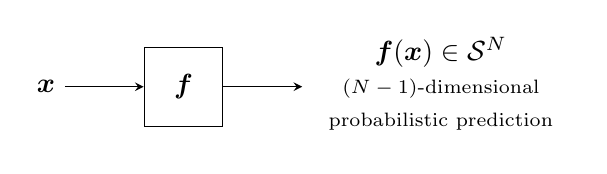
\begin{tikzpicture}
  \node [draw,
	minimum width=1cm,
	minimum height=1cm
        ]  (model) {$\bm{f}$};
        \node [left=1cm of model] (x) {$\bm{x}$};
        \node [right=1cm of model] (pred) {\begin{tabular}{c}$\bm{f}(\bm{x})\in \mathcal{S}^N$\\\scriptsize $(N-1)$-dimensional\\\scriptsize probabilistic prediction\end{tabular}};
        \draw[-stealth] (x.east) -- (model.west);
        \draw[-stealth] (model.east) -- (pred.west);
      \end{tikzpicture}
    \end{figure}

  \end{frame}

  \begin{frame}
    \frametitle{Shapley composition on the simplex}

    We rewrite the \textbf{prediction difference} and the \textbf{contribution} as follows:
    \begin{itemize}
      \pause
    \item \begin{equation}
        \begin{aligned}
          \bm{\delta}_{\bm{f},\bm{x},\text{Pr}}: 2^{\mathcal{I}} &\to \mathcal{S}^N,\\
          S &\mapsto \mathbb{E}^{\mathcal{A}}_\text{Pr}[\bm{f}(\bm{x})\mid \bm{x}_S] \ominus \mathbb{E}^{\mathcal{A}}_\text{Pr}[\bm{f}(\bm{x})],
        \end{aligned}
      \end{equation}
      \pause
      \item \begin{equation}
        \bm{c}_{\bm{f},\bm{x},\text{Pr}}(i,\bm{X}_S) = \bm{\delta}_{\bm{f},\bm{x},\text{Pr}}(\bm{X}_{S\cup\{i\}}) \ominus \bm{\delta}_{\bm{f},\bm{x},\text{Pr}}(\bm{X}_S),
      \end{equation}
    \end{itemize}
where $\bm{a}\ominus\bm{b}$ is the perturbation $\bm{a} \oplus \left( (-1)\odot \bm{b}\right)$ which correspond to a substraction between compositions $\bm{a}$ and $\bm{b}$, and where:
    
\end{frame}

\begin{frame}
  \frametitle{Shapley composition on the simplex}
  The Shapley quantity expressing the contribution of the $i$th feature on a prediction can simply be expressed on the simplex as the composition $\bm{\phi}(i)$ given by:
\begin{equation}
  \bm{\phi}_{\bm{f},\bm{x},\text{Pr}}(i) = \frac{1}{d!} \odot \underset{\pi}{\bigoplus}\bm{c}_{\bm{f},\bm{x},\text{Pr}}(i,\pi^{<i}_{\bm{X}}).
\end{equation}
We call this quantity {\large\textbf{Shapley composition}}.\\
It lives on the probability simplex.
\vspace{0.5cm}

\pause
It is:
\begin{itemize}
\item Linear 
\item Efficient: $\underset{i=1}{\overset{d}\bigoplus} \bm{\phi}_{\bm{f}}(i) = \bm{f}(\bm{x}) \ominus \mathbb{E}^{\mathcal{A}}_{\text{Pr}}[\bm{f}(\bm{X})]$
\item Symmetric
\end{itemize}

\end{frame}


\section{Explaining a prediction with Shapley compositions}

\begin{frame}
\frametitle{Explaining a prediction with Shapley compositions}
\framesubtitle{Visualizations in the isometric-log-ratio space}

We can visualize the Shapley compositions in the isometric-log-ratio space.
\begin{figure}
  \centering
  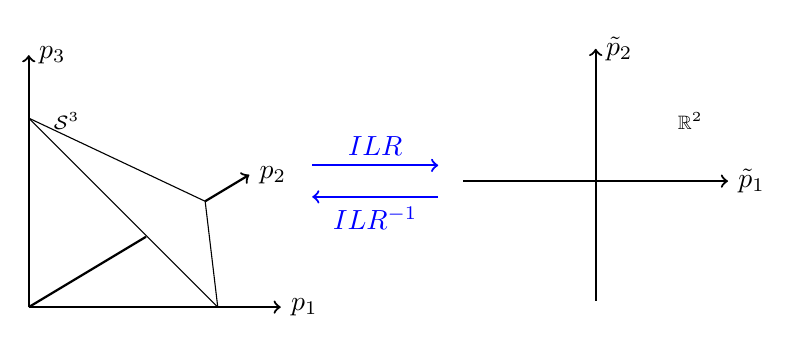
\begin{tikzpicture}[scale=0.8]

\draw [->,thick] (0,0) -- (0,4) node [right] {$p_3$};
\draw [->,thick] (0,0) -- (4,0) node [right] {$p_1$};
\draw [thick] (0,0) -- (1.86,1.116);
\draw [->,thick] (2.8,1.68) -- (3.5,2.1) node [right] {$p_2$};
\draw [] (0,3) -- (3,0);
\draw [] (0,3) -- (2.8,1.68);
\draw [] (3,0) -- (2.8,1.68);
\draw [] (0.6,2.95) node {\scriptsize $\mathcal{S}^3$};

\draw [->,thick,blue] (4.5,2.25) -- (6.5,2.25) node [pos=0.5,above] {$ILR$};
\draw [->,thick,blue] (6.5,1.75) -- (4.5,1.75) node [pos=0.5,below] {$ILR^{-1}$};

\draw [->,thick] (6.9,2) -- (11.1,2) node [right] {$\tilde{p}_1$};
\draw [->,thick] (9,0.1) -- (9,4.1) node [right] {$\tilde{p}_2$};
\draw [] (10.5,2.95) node {\scriptsize $\mathbb{R}^2$};

\end{tikzpicture}



%%% Local Variables:
%%% mode: latex
%%% TeX-master: "../main"
%%% End:

  \caption{Isometric-log-ratio transformation of the $2$-dimensional simplex (basis obtained with the Gram-Schmidt procedure)}
\end{figure}
where $\tilde{p}_1 = \frac{1}{\sqrt{2}} \log \frac{p_1}{p_2}$ and $\tilde{p}_2 = \frac{1}{\sqrt{6}} \log \frac{p_1p_2}{p_3^2}$.
\end{frame}

\begin{frame}
\frametitle{Explaining a prediction with Shapley compositions}
\framesubtitle{Visualizations in the isometric-log-ratio space}

And with more classes?
\vspace{0.2cm}

We can still visualize subspaces.
\pause
\begin{figure}
  \centering
  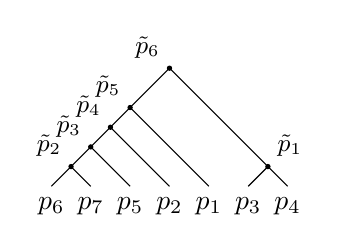
\begin{tikzpicture}[scale=1]
  \draw (0,0) -- (1.5,1.5);
  \draw (0.25,0.25) -- (0.5,0);
  \draw (0.5,0.5) -- (1,0);
  \draw (0.75,0.75) -- (1.5,0);
  \draw (1,1) -- (2,0);
  \draw (1.5,1.5) -- (3,0);
  \draw (2.75,0.25) -- (2.5,0);

  \filldraw[black] (0.25,0.25) circle (0.75pt) node[anchor=south east]{\small $\tilde{p}_{2}$};
  \filldraw[black] (0.5,0.5) circle (0.75pt) node[anchor=south east]{\small $\tilde{p}_{3}$};
  \filldraw[black] (0.75,0.75) circle (0.75pt) node[anchor=south east]{\small $\tilde{p}_{4}$};
  \filldraw[black] (1,1) circle (0.75pt) node[anchor=south east]{\small $\tilde{p}_{5}$};
  \filldraw[black] (1.5,1.5) circle (0.75pt) node[anchor=south east]{\small $\tilde{p}_{6}$};
  \filldraw[black] (2.75,0.25) circle (0.75pt) node[anchor=south west]{\small $\tilde{p}_{1}$};
  
  \draw[black] (0,-0.25) node{$p_6$};
  \draw[black] (0.5,-0.25) node{$p_7$};
  \draw[black] (1,-0.25) node{$p_5$};
  \draw[black] (1.5,-0.25) node{$p_2$};
  \draw[black] (2,-0.25) node{$p_1$};
  \draw[black] (2.5,-0.25) node{$p_3$};
  \draw[black] (3,-0.25) node{$p_4$};
\end{tikzpicture}


%%% Local Variables:
%%% mode: latex
%%% TeX-master: "main"
%%% End:

  \caption{Bifurcation tree used in our $10$-classes digit recognition task.}
\end{figure}
\end{frame}

\begin{frame}
  \frametitle{Explaining a prediction with Shapley compositions}
  \framesubtitle{Histograms}
  \begin{figure}
    \centering
    \includegraphics[width=0.9\linewidth]{../paper/figures/3classes/histo.png}
    \caption{Shapley compositions visualized as histograms
for the Iris classification example}
  \end{figure}
\end{frame}

\begin{frame}
  \frametitle{Explaining a prediction with Shapley compositions}
  \framesubtitle{Histograms}
  \begin{figure}
    \centering
    \includegraphics[width=0.9\linewidth]{../paper/figures/moreclasses/histo.png}
    \caption{Shapley compositions visualized as histograms for the seven classes digit recognition example.}
  \end{figure}
\end{frame}

\begin{frame}
  \frametitle{Explaining a prediction with Shapley compositions}

  \begin{center}
    Use the geometrical tools!
  \end{center}
  \vspace{0.2cm}
  
  We can summarize an explanation with:
  \begin{itemize}
  \item The norms of the Shapley compositions,
  \item Angles between them,
  \item And projection on the class-compositions.
  \end{itemize}
\end{frame}

\section{Discussion and conclusion}

\begin{frame}
\frametitle{Discussion and conclusion}
Summarize:
\begin{itemize}
\item We proposed an extention of the concept of Shapley value for explaination in a multiclass setting
\pause
\item Shapley composition,
\pause
\item \st{scalar} \textbf{distribution/composition} living on the simplex
  \pause
\item Visualisations in the ILR space, or as histograms,
  \pause
  \item Computation of norms, angles and projections.
\end{itemize}

\pause
\vspace{0.2cm}
Future work:
\begin{itemize}
\item The literature about Shapley value is prolific,
\pause
\item Axiomatic formulation and uniqueness...
\end{itemize}
\end{frame}


\begin{frame}[t,allowframebreaks]
   \frametitle{References}
    \printbibliography
  \end{frame}


\begin{frame}
\frametitle{Thank you!!}
\begin{figure}\centering
  \includegraphics[width=0.6\linewidth]{bowling.JPG}
\end{figure}


\end{frame}



\end{document}
%%% Local Variables:
%%% mode: latex
%%% TeX-master: t
%%% End:
